\chapter{Что такое OTP?}
\label{what-is-otp}
\section{Это Открытая Телекоммуникационная Платформа!}
\label{its-the-open-telecom-platform}
\begin{wrapfigure}{l}{0.35\linewidth}
    
\includegraphics[width=1\linewidth]{hullo.png}
    ВОПРОС ИСХОДИТ ИЗ ДОМА
\end{wrapfigure}
OTP можно расшифровать как \emph{Открытая Телекоммуникационная Платформа}, хотя с телекоммуникациями она уже не так сильно связана, как прежде (она больше связана с программами, которые решают задачи, характерные для сферы телекоммуникаций).
Если сказать, что половина величия Erlang заключена в его параллелизме (concurrency) и распределённости, а вторая половина \--- в его средствах обработки ошибок, то третьей половиной будет OTP фреймворк.

В предыдущих главах мы рассмотрели несколько примеров общих правил, которым следуют при создании параллельных (concurrent) приложений, применяя встроенные средства языка: связи (links), мониторы, серверы, таймауты, улавливающие завершения (trapping exits), и т.д.
То и дело мы натыкались на подводные камни, и придумывали пути их обхода.
Размышляли о том, как избежать состояний гонки (race conditions), и о том, как важно не забывать, что процесс может умереть в любой момент.
Мы также столкнулись с горячей загрузкой кода, именованием процессов и применением супервизоров.

Если делать всё перечисленное вручную, приходится тратить много времени, а ошибку при этом можно допустить очень легко.
Есть немало граничных случаев, о которых можно забыть, и множество ловушек, в которые легко угодить.
Фреймворк OTP справляется с этой задачей, группируя жизненно важные принципы в набор библиотек, которые подверглись тщательной проектировке и годами закалялись в боях.
Их должен использовать каждый программист на Erlang.

Фреймворк OTP также включает набор модулей и стандартов, призванных помогать разработчику в построении приложения.
Если допустить, что большинство программистов на Erlang в конце концов приходят к использованию OTP, то большинство приложений, с которыми вы сможете столкнуться, будут склонны к следованию этим стандартам. 
\section{Обычный процесс в обобщении}
\label{the-common-process-abstracted}
Одним из общих приёмов, который мы многократно применяли в предыдущих примерах с процессами, было разделение всего что только можно в соответствии с очень конкретными задачами.
В большинстве процессов имеется функция, отвечающая за порождение нового процесса \--- функция, которая заведовала выдачей процессу начальных значений, основного цикла и т.д.

Оказывается, эти части обычно присутствуют во всех параллельных (concurrent) программах, которые вы будете писать, не взирая на назначение процесса.
\begin{figure}[h!]
    \centering
    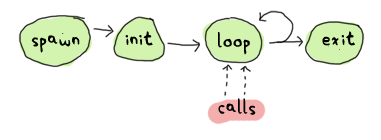
\includegraphics[width=0.7\textwidth]{common-pattern.png}
\end{figure}

Инженеры и учёные, которые занимались разработкой OTP, выявили такие шаблоны и включили их в состав нескольких простых библиотек.
Эти библиотеки содержат код, эквивалентный большинству абстракций, использованных нами (таких, например, как пометка сообщений ссылками).
Но код этот выгодно отличается от нашего тем, что на протяжении многих лет его применяют в боевых условиях, и он был построен с намного большей предусмотрительностью, чем наша реализация.
В состав библиотек входят функции для безопасного порождения и инициализации процессов, отсылки сообщений с устойчивостью к сбоям и многое другое.
Забавно то, что вам редко придётся использовать эти библиотеки самостоятельно.
Абстракции, которые они содержат, настолько просты и универсальны, что на их основе были построены намного более интересные штуки.
Вот именно библиотеками, которые содержат такие штуки, мы и воспользуемся.
\begin{figure}[h!]
    \centering
    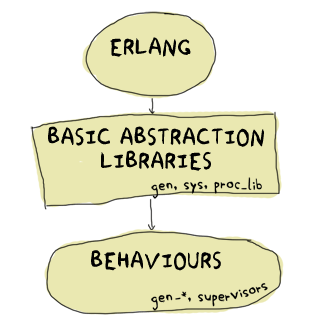
\includegraphics[width=0.65\textwidth]{abstraction-layers.png}
\end{figure}
В последующих главах мы столкнёмся с несколькими распространёнными вариантами использования процессов, а затем увидим как их можно обобщить и сделать универсальными.
Затем мы рассмотрим реализацию каждого из этих приёмов с помощью шаблонов поведения фреймворка OTP (OTP framework's behaviours), и увидим как их можно применять.
\section{Базовый сервер}
\label{the-basic-server}
Первым общепринятым шаблоном, который я опишу, мы уже успели воспользоваться.
При написании \ref{designing-a-concurrent-application} сервера событий, мы использовали то, что можно назвать \emph{моделью клиент\--сервер}.
Сервер событий получает вызовы от клиента, обрабатывает их и формирует ответы, если того требует протокол.

Для этой главы мы будем использовать очень простой сервер, который позволит нам сконцентрироваться на его основных свойствах.
Вот как выглядит \href{http://learnyousomeerlang.com/static/erlang/kitty\_server.erl}{котосервер}
\begin{lstlisting}[style=erlang]
%%%%% Naive version
-module(kitty_server).
 
-export([start_link/0, order_cat/4, return_cat/2, close_shop/1]).
 
-record(cat, {name, color=green, description}).
 
%%% Client API
start_link() -> spawn_link(fun init/0).
 
%% Synchronous call
order_cat(Pid, Name, Color, Description) ->
    Ref = erlang:monitor(process, Pid),
    Pid ! {self(), Ref, {order, Name, Color, Description}},
    receive
        {Ref, Cat} ->
            erlang:demonitor(Ref, [flush]),
            Cat;
        {'DOWN', Ref, process, Pid, Reason} ->
            erlang:error(Reason)
    after 5000 ->
        erlang:error(timeout)
    end.
 
%% This call is asynchronous
return_cat(Pid, Cat = #cat{}) ->
    Pid ! {return, Cat},
    ok.
 
%% Synchronous call
close_shop(Pid) ->
    Ref = erlang:monitor(process, Pid),
    Pid ! {self(), Ref, terminate},
    receive
        {Ref, ok} ->
            erlang:demonitor(Ref, [flush]),
            ok;
        {'DOWN', Ref, process, Pid, Reason} ->
            erlang:error(Reason)
    after 5000 ->
        erlang:error(timeout)
    end.
 
%%% Server functions
init() -> loop([]).
 
loop(Cats) ->
    receive
        {Pid, Ref, {order, Name, Color, Description}} ->
            if Cats =:= [] ->
                Pid ! {Ref, make_cat(Name, Color, Description)},
                loop(Cats);
            Cats =/= [] -> % got to empty the stock
                Pid ! {Ref, hd(Cats)},
                loop(tl(Cats))
            end;
        {return, Cat = #cat{}} ->
            loop([Cat|Cats]);
        {Pid, Ref, terminate} ->
            Pid ! {Ref, ok},
            terminate(Cats);
        Unknown ->
            %% do some logging here too
            io:format("Unknown message: ~p~n", [Unknown]),
            loop(Cats)
    end.
 
%%% Private functions
make_cat(Name, Col, Desc) ->
    #cat{name=Name, color=Col, description=Desc}.
 
terminate(Cats) ->
    [io:format("~p was set free.~n",[C#cat.name]) || C <- Cats],
    ok.
\end{lstlisting}

Такой вот котосервер/магазин.
Его поведение чрезвычайно незатейливо: вы описывает кота и вы этого кота получаете.
Если кота вернули назад, он попадает в список, и затем автоматически высылается в следующем заказе, не принимая во внимание то, что фактически запросил клиент (мы же деньги зарабатываем, а не шутки шутим): \begin{lstlisting}[style=erlang]
1> c(kitty_server). 
{ok,kitty_server}
2> rr(kitty_server).
[cat]
3> Pid = kitty_server:start_link().
<0.57.0>
4> Cat1 = kitty_server:order_cat(Pid, carl, brown, "loves to burn bridges").
#cat{name = carl,color = brown,
    description = "loves to burn bridges"}
5> kitty_server:return_cat(Pid, Cat1).
ok
6> kitty_server:order_cat(Pid, jimmy, orange, "cuddly").
#cat{name = carl,color = brown,
    description = "loves to burn bridges"}
7> kitty_server:order_cat(Pid, jimmy, orange, "cuddly").
#cat{name = jimmy,color = orange,description = "cuddly"}
8> kitty_server:return_cat(Pid, Cat1).
ok
9> kitty_server:close_shop(Pid).
carl was set free.
ok
10> kitty_server:close_shop(Pid).
** exception error: no such process or port
    in function  kitty_server:close_shop/1
\end{lstlisting}

Вернёмся к исходному коду модуля.
В нём можно заметить шаблоны, которые мы применяли ранее.
Видны участки кода, где мы включали и выключали мониторы, применяли таймеры, получали данные, использовали основной цикл, управляли функцией инициализации и т.д.
Всё это должно быть нам знакомо.
Наверняка все эти вещи, которые мы постоянно повторяем, можно как\--то обобщить.

Для начала давайте поглядим на API клиента.
Сразу в глаза бросается то, что оба синхронных вызова очень похожи друг на друга.
Эти вызовы наверняка могли попасть в обобщённые библиотеки, о которых я упоминал в предыдущем разделе.
Пока что мы просто выразим эти вызовы в виде одной функции, которая станет частью \href{http://learnyousomeerlang.com/static/erlang/my\_server.erl}{нового модуля}, объединяющего все обобщённые части котосервера:
\begin{lstlisting}[style=erlang]
-module(my_server).
-compile(export_all).
 
call(Pid, Msg) ->
    Ref = erlang:monitor(process, Pid),
    Pid ! {self(), Ref, Msg},
    receive
        {Ref, Reply} ->
            erlang:demonitor(Ref, [flush]),
            Reply;
        {'DOWN', Ref, process, Pid, Reason} ->
            erlang:error(Reason)
    after 5000 ->
        erlang:error(timeout)
    end.
\end{lstlisting}

Код принимает сообщение и PID, запихивает их в функцию, а затем пересылает это сообщение безопасным методом.
С этого момента мы сможем просто заменять пересылку сообщения вызовом этой функции.
И если бы мы переписали заново котосервер, чтобы он связывался с обобщённым \ops{my\_server}, его начало могло бы выглядеть так:
\begin{lstlisting}[style=erlang]
-module(kitty_server2).
-export([start_link/0, order_cat/4, return_cat/2, close_shop/1]).
 
-record(cat, {name, color=green, description}).
 
%%% Client API
start_link() -> spawn_link(fun init/0).
 
%% Synchronous call
order_cat(Pid, Name, Color, Description) ->
    my_server:call(Pid, {order, Name, Color, Description}).
 
%% This call is asynchronous
return_cat(Pid, Cat = #cat{}) ->
    Pid ! {return, Cat},
    ok.
 
%% Synchronous call
close_shop(Pid) ->
    my_server:call(Pid, terminate).
\end{lstlisting}
Следующий типовой кусок кода, который требует нашего внимания, не выглядит так же просто как функция \ops{call/2}.
Обратите внимание, что все процессы, написанные нами до этого момента, содержат в себе цикл, в котором производится сопоставление с образцом для всех полученных сообщений.
Сейчас мы сделаем немного рискованный шаг, и попробуем отделить сопоставление с образцом от, собственно, самого цикла.
Одним из способов реализации может оказаться такой:
\begin{lstlisting}[style=erlang]
loop(Module, State) ->
    receive
        Message -> Module:handle(Message, State)
    end.
\end{lstlisting}

А сам модуль может выглядеть так:
\begin{lstlisting}[style=erlang]
handle(Message1, State) -> NewState1;
handle(Message2, State) -> NewState2;
...
handle(MessageN, State) -> NewStateN.
\end{lstlisting}
Вот.
Уже лучше.
Но можно сделать этот код ещё более понятным.
Если вы внимательно читали код модуля \ops{kitty\_server} (а я надеюсь, что так оно и было!), вы должны были заметить, что у нас заведен определённый порядок выполнения синхронных вызовов, а асинхронные вызовы мы совершаем совсем иначе.
Было бы весьма неплохо, если бы наша реализация типового сервера могла предоставлять ясное средство для определения типа вызова, с которым мы имеем дело.

Чтобы создать такую возможность, нам нужно будет проводить сопоставление  в функции \ops{my\_server:loop/2} с различными видами сообщений.
Поэтому нам придётся немного изменить вторую строку функции \ops{call/2}, чтобы синхронные вызовы ясно обозначались при помощи добавления в сообщение атома \ops{sync}:
\begin{lstlisting}[style=erlang]
call(Pid, Msg) ->
    Ref = erlang:monitor(process, Pid),
    Pid ! {sync, self(), Ref, Msg},
    receive
        {Ref, Reply} ->
            erlang:demonitor(Ref, [flush]),
            Reply;
        {'DOWN', Ref, process, Pid, Reason} ->
            erlang:error(Reason)
    after 5000 ->
        erlang:error(timeout)
    end.
\end{lstlisting}

Теперь мы можем создать новую функцию для асинхронных вызовов.
Этим будет заниматься \ops{cast/2}:
\begin{lstlisting}[style=erlang]
cast(Pid, Msg) ->
    Pid ! {async, Msg},
    ok.
\end{lstlisting}
С этими изменениями цикл будет выглядеть так:
\begin{lstlisting}[style=erlang]
loop(Module, State) ->
    receive
        {async, Msg} ->
            loop(Module, Module:handle_cast(Msg, State));
        {sync, Pid, Ref, Msg} ->
            loop(Module, Module:handle_call(Msg, Pid, Ref, State))
    end.
\end{lstlisting}
А потом можно ещё добавить выделенные слоты для обработки сообщений, которые не вписываются в концепцию синхронности/асинхронности (может быть их послали случайно), и туда же можно добавить функции отладки и всё прочее, например, горячую перезагрузку кода.
\begin{wrapfigure}{r}{0.35\linewidth}
    
\includegraphics[width=1\linewidth]{sink.png}
    Поняли намёк? ПОНЯЛИ?
\end{wrapfigure}

В вышеприведённом цикле есть один досадный момент: абстракция раскрывает своё внутреннее устройство (протекающая абстракция, leaking abstraction).
Тем программистам, которые воспользуются \ops{my\_server} для отправки синхронных сообщений и ответа на них, нужно будет иметь представление о ссылках.
Из\--за этого абстракция теряет всякий смысл.
Чтобы использовать такой код, вам всё равно придётся понимать все скучные подробности его реализации.
Вот как мы можем это быстро исправить:
\begin{lstlisting}[style=erlang]
loop(Module, State) ->
    receive
        {async, Msg} ->
            loop(Module, Module:handle_cast(Msg, State));
        {sync, Pid, Ref, Msg} ->
            loop(Module, Module:handle_call(Msg, {Pid, Ref}, State))
    end.
\end{lstlisting}

Поместив обе переменные \emph{Pid} и \emph{Ref} в кортеж, мы сможем передавать их в другие функции как один аргумент, например как переменную с именем \emph{From}.
И пользователь ничего не должен знать о внутренностях этой переменной.
Мы также предоставим функцию для отсылки ответов, которая будет понимать содержимое \emph{From}:
\begin{lstlisting}[style=erlang]
reply({Pid, Ref}, Reply) ->
    Pid ! {Ref, Reply}.
\end{lstlisting}

Осталось только указать запускающие функции (\ops{start}, \ops{start\_link} и \ops{init}), которые передают друг другу имена модулей и всякие мелочи.
После их добавления, модуль примет следующий вид:
\begin{lstlisting}[style=erlang]
-module(my_server).
-export([start/2, start_link/2, call/2, cast/2, reply/2]).
 
%%% Public API
start(Module, InitialState) ->
    spawn(fun() -> init(Module, InitialState) end).
 
start_link(Module, InitialState) ->
    spawn_link(fun() -> init(Module, InitialState) end).
 
call(Pid, Msg) ->
    Ref = erlang:monitor(process, Pid),
    Pid ! {sync, self(), Ref, Msg},
    receive
        {Ref, Reply} ->
            erlang:demonitor(Ref, [flush]),
            Reply;
        {'DOWN', Ref, process, Pid, Reason} ->
            erlang:error(Reason)
    after 5000 ->
        erlang:error(timeout)
    end.
 
cast(Pid, Msg) ->
    Pid ! {async, Msg},
    ok.
 
reply({Pid, Ref}, Reply) ->
    Pid ! {Ref, Reply}.
 
%%% Private stuff
init(Module, InitialState) ->
    loop(Module, Module:init(InitialState)).
 
loop(Module, State) ->
    receive
        {async, Msg} ->
            loop(Module, Module:handle_cast(Msg, State));
        {sync, Pid, Ref, Msg} ->
            loop(Module, Module:handle_call(Msg, {Pid, Ref}, State))
    end.
\end{lstlisting}

Далее мы перепишем котосервер.
Теперь \href{http://learnyousomeerlang.com/static/erlang/kitty\_server2.erl}{kitty\_server2} будет выступать вызываемым модулем (callback module), который будет соответствовать интерфейсу, определённому нами для \ops{my\_server}.
Мы сохраним тот же интерфейс, что использовался в предыдущей реализации, но теперь все вызовы будут перенаправляться для прохождения через \ops{my\_server}:
\begin{lstlisting}[style=erlang]
-module(kitty_server2).
 
-export([start_link/0, order_cat/4, return_cat/2, close_shop/1]).
-export([init/1, handle_call/3, handle_cast/2]).
 
-record(cat, {name, color=green, description}).
 
%%% Client API
start_link() -> my_server:start_link(?MODULE, []).
 
%% Synchronous call
order_cat(Pid, Name, Color, Description) ->
    my_server:call(Pid, {order, Name, Color, Description}).
 
%% This call is asynchronous
return_cat(Pid, Cat = #cat{}) ->
    my_server:cast(Pid, {return, Cat}).
 
%% Synchronous call
close_shop(Pid) ->
    my_server:call(Pid, terminate).
\end{lstlisting}

Обратите внимание, что я добавил второй \ops{-export()} в заголовок модуля.
Там указаны функции, которые должны вызываться \ops{my\_server}\--ом для корректной работы:
\begin{lstlisting}[style=erlang]
%%% Server functions
init([]) -> []. %% no treatment of info here!
 
handle_call({order, Name, Color, Description}, From, Cats) ->
    if Cats =:= [] ->
         my_server:reply(From, make_cat(Name, Color, Description)),
         Cats;
        Cats =/= [] ->
         my_server:reply(From, hd(Cats)),
         tl(Cats)
    end;
 
handle_call(terminate, From, Cats) ->
    my_server:reply(From, ok),
    terminate(Cats).
 
handle_cast({return, Cat = #cat{}}, Cats) ->
    [Cat|Cats].
\end{lstlisting}

А теперь нужно повторно добавить закрытые (private) функции:
\begin{lstlisting}[style=erlang]
%%% Private functions
make_cat(Name, Col, Desc) ->
    #cat{name=Name, color=Col, description=Desc}.
 
terminate(Cats) ->
    [io:format("~p was set free.~n",[C#cat.name]) || C <- Cats],
    exit(normal).
\end{lstlisting}

Главное, убедитесь, что заменили \ops{ok}, который мы использовали раньше, на \ops{exit(normal)} в функции \ops{terminate/1}, иначе сервер не будет завершаться.

Этот код должен компилироваться, тестироваться и запускаться совершенно так же как и раньше.
Выглядит он очень похоже, но давайте рассмотрим подробнее, что же поменялось.
\section{Частное против общего}
\label{specific-vs-generic}
Только что мы пришли к пониманию сути OTP (как концепции).
Вот для чего на самом деле существует OTP: мы берём общие компоненты, извлекаем их и помещаем в библиотеки, при этом следим, чтобы они правильно работали, а затем по возможности стараемся использовать этот код повторно.
Осталось только сконцентрироваться на частном, на том, что будет меняться от приложения к приложению.

Очевидно, что применяя эти приёмы лишь к котосерверу, большого преимущества нам не видать.
Может даже возникнуть впечатление, что мы создаём абстракцию ради самой абстракции.
Если бы приложение, которое мы должны разработать для клиента, состояло из одного лишь котосервера, то мы могли бы остановиться на первой версии.
Но если вы намерены иметь дело с приложениями побольше, то, вероятно, имеет смысл отделить общие участки кода от частных.

Давайте представим на мгновение, что на нашем сервере запущена некоторая программа на Erlang.
В этой программе запускается несколько котосерверов, ветеринарный процесс (вы пересылаете ему сломанных кошечек, а он их возвращает в исправном состоянии), кошачий салон красоты, сервер еды для домашних животных, склад с припасами и т.д.
Большинство из этих задач можно реализовать при помощи шаблона клиент\--сервер.
Но с течением времени вашу сложную систему заполоняет множество различных действующих серверов.

Чем больше серверов, тем сложнее код, его тестирование, поддержка и осмысление.
Каждая реализация может отличаться от другой, может быть запрограммирована в разных стилях разными людьми и так далее.
Но если все эти серверы следуют единой абстракции, определённой в \ops{my\_server}, мы существенно уменьшаем эту сложность.
Вам сразу же становится понятна общая концепция, положенная в основу модуля (<<о, так это же сервер!>>), у него существует единая общая канва, согласно которой можно проводить тестирование, писать документацию и т.д.
Остаток усилий можно приложить к особенностям каждой конкретной реализации.

\begin{wrapfigure}{r}{0.35\linewidth}
    
\includegraphics[width=1\linewidth]{dung.png}
    Это я двигаю код в продакшен
\end{wrapfigure}

Таким образом вы сможете сократить время, затраченное на отслеживание и исправление ошибок (можно всё это просто делать в одном месте для всех серверов).
Вдобавок вы уменьшите количество ошибок, которые вносите в код программы.
Если бы вам каждый раз приходилось переписывать функцию \ops{my\_server:call/3}, или главный цикл программы, то это бы не только потребовало больших затрат времени, но и чрезвычайно увеличило бы шансы на пропуск того или иного шага, и поспособствовало появлению ошибок.
Чем меньше ошибок, тем меньше ночных звонков с требованием что\--либо исправить, а это наверняка всем придётся по душе.
Может быть вы придерживаетесь иного мнения, но готов поспорить, что навещать офис в нерабочий день для исправления ошибок вам тоже не особенно хочется.

Ещё одним интересным улучшением, которое мы сделали, разделив общее и частное, является значительное облегчение тестирования отдельных модулей.
Если бы вы захотели провести юнит\--тестирование старой реализации котосервера, вам бы понадобилось порождать на каждый тест по отдельному процессу, наделять его правильным состоянием, посылать сообщения и надеяться на получение необходимого ответа.
Наш второй котосервер, напротив, требует лишь вызова функций 'handle\_call/3' и 'handle\_cast/2', и обработки возвращаемого нового состояния.
Не нужно настраивать серверы, манипулировать состоянием.
Нужно просто передать его функции в качестве входного параметра.
Следует отметить, что это также облегчает тестирование общей части сервера.
Вам просто нужно реализовать несколько очень простых функций, которые изолированно позволяют пронаблюдать за тестируемым поведением, не обращая внимание на всё остальное.

К намного более <<незаметным>> преимуществам использования общих абстракций можно отнести то, что если все используют совершенно одинаковый бэкенд для своих процессов, то после оптимизации этого единого бэкенда, каждый использующий его процесс получит прирост в производительности.
Чтобы этот принцип работал на практике, многие люди должны вкладывать усилия в использование одних и тех же абстракций.
К счастью, в Erlang\--сообществе это требование выполняется для фреймворка OTP.

Вернёмся к нашим модулям.
Мы ещё не успели обсудить много вещей: именованные процессы, конфигурация тайм\--аутов, добавление отладочной информации, что делать с неожиданными сообщениями, как встроить горячую загрузку кода, как обработать некоторые особенные ошибки, как обобщить код необходимый для ответа на сообщения, как управлять завершением сервера, чтобы он правильно взаимодействовал с супервизорами и т.д.
Все эти темы избыточны для данного руководства, но совершенно необходимы в настоящих программных продуктах.
И снова вы можете заметить, что самостоятельное решение всех этих проблем может оказаться несколько рискованным мероприятием.
К счастью для вас (и для людей, которые будут поддерживать ваше приложение), команда Erlang/OTP смогла справиться со всеми перечисленными проблемами при помощи шаблона поведения gen\_server.
\ops{gen\_server} напоминает \ops{my\_server} на стероидах, с тем лишь отличием, что за его плечами стоят многие годы тестирования и применения в рабочей среде.
